\documentclass[polish,a4paper]{article}
\usepackage[utf8]{inputenc}
\usepackage[T1]{fontenc}
%%\usepackage{polski}
\usepackage{amsmath}
\usepackage{amssymb,amsfonts,amsthm}
\usepackage{babel}
\usepackage{hyperref}
\usepackage{xcolor}
\usepackage{graphicx} 
\usepackage{caption}
\usepackage{subcaption}
\usepackage{listings}
\usepackage{anysize}
%%\usepackage{tabto}

\graphicspath{ {img/} }
\marginsize{2.5cm}{2.5cm}{0cm}{3cm}

\definecolor{codegreen}{rgb}{0,0.6,0}
\definecolor{codegray}{rgb}{0.5,0.5,0.5}
\definecolor{codepurple}{rgb}{0.58,0,0.82}
\definecolor{backcolour}{rgb}{0.95,0.95,0.92}

\lstdefinestyle{mystyle}{
	backgroundcolor=\color{backcolour},   
	commentstyle=\color{codegreen},
	keywordstyle=\color{magenta},
	numberstyle=\tiny\color{codegray},
	stringstyle=\color{codepurple},
	basicstyle=\ttfamily\footnotesize,
	breakatwhitespace=false,         
	breaklines=true,                 
	captionpos=b,                    
	keepspaces=true,                 
	numbers=left,                    
	numbersep=5pt,                  
	showspaces=false,                
	showstringspaces=false,
	showtabs=false,                  
	tabsize=2
}

\lstset{style=mystyle}

\begin{document}
	\begin{center}
		\begin{tabular}{ p{0.32\textwidth} p{0.15\textwidth} p{0.15\textwidth} p{0.12\textwidth} p{0.12\textwidth} }
			
			&   &   &   &  \\
			\hline
			\multicolumn{5}{|c|}{}\\[-1ex]
			\multicolumn{5}{|c|}{{\LARGE \textbf{Laboratorium z przedmiotu Systemy wbudowane (SW)}}}\\
			\multicolumn{5}{|c|}{}\\[-1ex]
			\hline
			\hline
			
			\multicolumn{5}{|c|}{}\\[-1ex]
			\multicolumn{5}{|c|}{{\LARGE Zadanie nr 6}}\\
			\multicolumn{5}{|c|}{}\\[-1ex]
			\hline
			\hline
			
			\multicolumn{5}{|c|}{}\\[-1ex]
			\multicolumn{5}{|c|}{{\textbf{Temat zajęć:} BeagleBone Black – komunikacja}}\\
			\multicolumn{5}{|c|}{}\\[-1ex]
			\hline
			\hline
			
			\multicolumn{1}{|l|}{Prowadzący} &
			\multicolumn{2}{|l|}{Autorzy} &
			\multicolumn{1}{|l|}{Grupa dziekańska:}
			&
			\multicolumn{1}{|l|}{I1.2} \\
			\multicolumn{1}{|c|}{mgr inż. Ariel Antonowicz} &
			\multicolumn{2}{|c|}{148088 i 148121} &
			\multicolumn{1}{|c|}{\textbf{Ocena:}} &
			\multicolumn{1}{|c|}{}\\
			\hline
			\hline
		\end{tabular}
	\end{center}
	\[\,\]
	\section{Komunikacja}
	\begin{figure}[h!]
		\begin{center}
			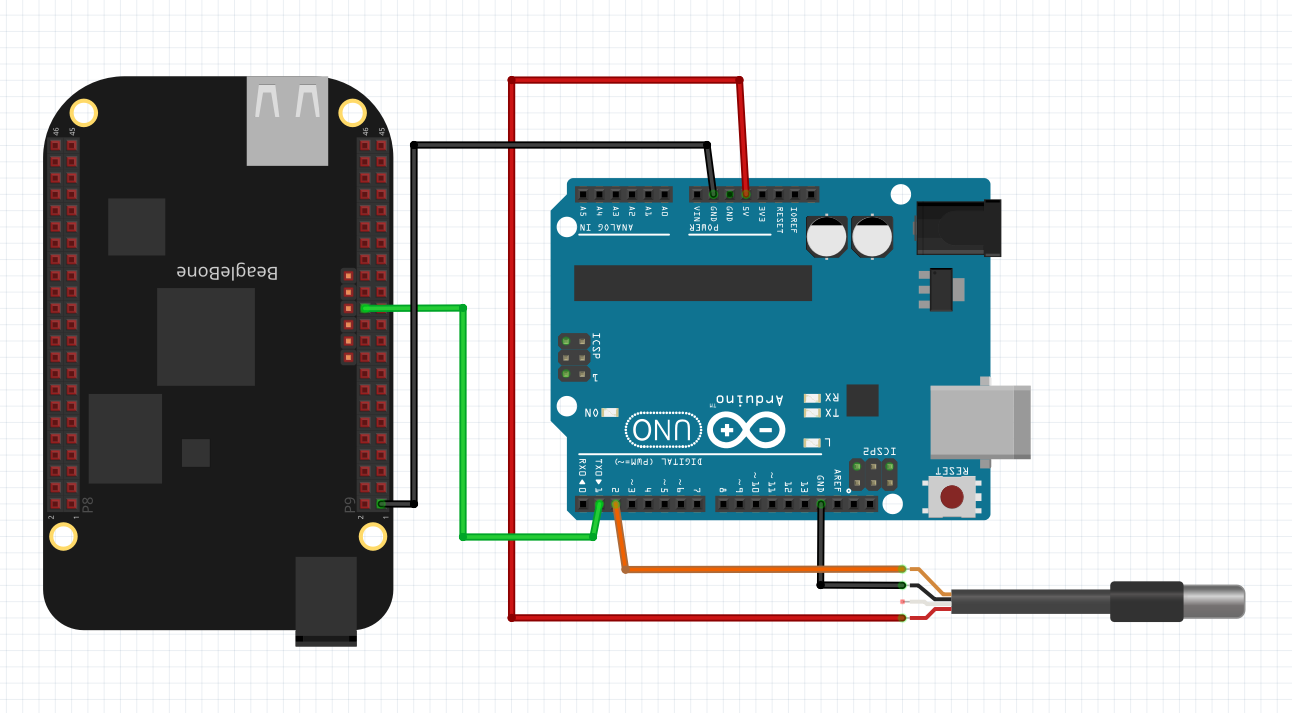
\includegraphics[scale=0.55]{UART.png}
			\caption*{Schemat podłączenia Arduino i BeagleBone'a za pomocą UART}
		\end{center}
	\end{figure}
	\newpage
	%,basicstyle=\scriptsize
	\begin{figure}[h!]
		\begin{lstlisting}[language=C++]
			#include <OneWire.h>
			#include <DS18B20.h>
			#include <SPI.h>
			#include <MFRC522.h>
			
			#define ONEWIRE_PIN 2
			
			// Adres czujnika
			byte address[8] = {0x28, 0xFF, 0xBC, 0x88, 0x90, 0x17, 0x5, 0x76};
			
			OneWire onewire(ONEWIRE_PIN);
			DS18B20 sensors(&onewire);
			
			int sort_desc(const void *cmp1, const void *cmp2){
				int a = *((int *)cmp1);
				int b = *((int *)cmp2);
				return a > b ? -1 : (a < b ? 1 : 0);
			}
			
			void setup() {
				while(!Serial);
				Serial.begin(9600);
				SPI.begin();      // Initiate  SPI bus
				sensors.begin();
				sensors.request(address);
			}
			
			void loop() {
				float vec[20];
				if (sensors.available())
				{
					for (int i = 0; i < 18; i++) {
						vec[i] = sensors.readTemperature(address);
					}
					qsort(vec, 18, sizeof(float), sort_desc);
					
					float sum = 0;
					for (int i = 1; i < 17; i++) {
						sum += vec[i];
					}
					sum /= 16;
					
					Serial.print(sum);
					Serial.println(F(" 'C"));
					sensors.request(address);
				}
			}
			
		\end{lstlisting}
		\caption*{Kod odpowiedzialny za odczytywanie danych z sensora oraz przesyłanie na port szeregowy przez Arduino (lab2)}
	\end{figure}
	
	
	\newpage
	
	\begin{figure}[h!]
		\begin{lstlisting}[language=Python]
			#!/usr/bin/python
			import Adafruit_DHT
			import datetime
			import sqlite3
			from sqlite3 import Error
			import Adafruit_BBIO.UART as UART
			import serial
			
			def create_connection(db):
			con = None
			try:
			con = sqlite3.connect(db)
			except Error as e:
			print(e)
			return con
			
			
			def create_table(con, create_sql):
			try:
			c = con.cursor()
			c.execute(create_sql)
			c.close()
			except Error as e:
			print(e)
			
			
			def insert2db(con, val):
			sql_insert = "INSERT INTO measurements(temp, date) VALUES(?,?)"
			cur = con.cursor()
			cur.execute(sql_insert, val)
			con.commit()
			cur.close()
			
			
			def return_table(con):
			cur = con.cursor()
			cur.execute("SELECT * from measurements")
			rows = cur.fetchall()
			for row in rows:
			print(row)
			cur.close()
			
			
			conn = create_connection('pysqlite.db')
			sql_create = "CREATE TABLE IF NOT EXISTS measurements (id INTEGER PRIMARY KEY AUTOINCREMENT, temp REAL, date TIMESTAMP);"
			create_table(conn, sql_create)    
		\end{lstlisting}
		\caption*{Importy bibliotek i funkcje do komunikacji z bazą danych - BeagleBone (lab5)}
	\end{figure}
	
	\newpage
	
	\begin{figure}[h!]
		\begin{lstlisting}[language=Python]
			UART.setup("UART1")
			
			ser = serial.Serial(port = "/dev/ttyO1", baudrate=9600)
			ser.close()
			ser.open()
			
			read = True
			
			if read:
			while True:
			if ser.isOpen():
			t = float(ser.readline().decode().split(' ')[0])  # byte strings to unicode
			if t is not None:
			# print(t)
			d = datetime.datetime.now()
			values = (t, d)
			insert2db(conn, values)
			else:
			print('Failed to get reading. Try again!')
		\end{lstlisting}
		\caption*{Odbieranie danych z UART oraz dodawnie ich do bazy danych sqlite}
	\end{figure}
	
	
	\section*{Źródła}
	\begin{enumerate}
		\item \href{https://forum.fritzing.org/}{Fritzing}
		\item Materiały podane przez prowadzącego na platformie ekursy.
		\item Sprawozdania z lab2 oraz lab5.
		\item \href{https://www.teachmemicro.com/beaglebone-black-serial-arduino/}{teachmemicro.com} 
		\item \href{https://www.pythonpool.com/python-serial-read/}{pythonpool.com}
	\end{enumerate}
	\begingroup
	\hypersetup{hidelinks}
	\tableofcontents
	\endgroup
\end{document}
